% anexo_a.tex

% International Carbon Action Partnership (ICAP). (2022). EU Emissions Trading System (EU ETS) Factsheet. ICAP. 

% Citizens Budget Commission of New York. (2023). Keys to a cap-and-invest design that’s earth- and economy-focused: Recommendations for a cost-effective program to meet New York's ambitious climate goals. https://cbcny.org/research/keys-cap-and-invest-design-thats-earth-and-economy-focused

\chapter{Anexos}
\label{}


% \section*{Propuesta de Hitos}

% \subsection*{Estructura Tesis}
% \paragraph{Resumen}
% \begin{itemize}
%     \item Se irán agregando los puntos claves del documento en este resumen a medida que se vayan haciendo
% \end{itemize}
% \paragraph{Introducción}
% \begin{itemize}
%     \item \textbf{Contexto global y nacional:}  
%     ¿Qué es el sistema Cap-and-Trade y por qué es importante para reducir las emisiones de carbono?

%     \item \textbf{Contexto hacia la investigación:}  
%     ¿Importa tener más información?  
%     ¿Es relevante invertir en información para que un subastador estime mejor un CAP?  
%     ¿Qué ocurre si el CAP no es del todo preciso?
% \end{itemize}

% \paragraph{Objetivos}
% \begin{itemize}
%     \item \textbf{Objetivo general:}  
%     Desarrollar y evaluar una reformulación del problema del subastador dentro de un modelo de equilibrio de Cap-and-Trade (basado en el trabajo de \citeA{amigo_two_2021} y tesis de Vicente), que incorpore la racionalidad del planificador social en la inversión en información para mejorar la precisión del límite de emisiones (CAP) y reducir el costo social asociado a desviaciones respecto al CAP óptimo o real.
    
%     \item \textbf{Objetivos específicos:}
%     \begin{enumerate}
%         \item Obtener los limites para el CAP que hacen sentido en Chile, por medio de investigación.
%         \item Reconocer qué variables y parámetros realizados en la tesis de Vicente serán útiles para la mía. Analizar si alguna variable será considerada cómo parámetro o viceversa, y si tendré que agregar o quitar a una de estas.
%         \item Plantear matemáticamente cuándo deja de ser óptimo invertir en información.
%         \item Modelar el problema en Julia y evaluar los resultados de manera coherente.
%     \end{enumerate}
% \end{itemize}

% \paragraph{Alcances}
% Se abordará la inversión en información por parte del subastador para encontrar un óptimo en el CAP estimado y analizar cómo esto afecta a la sociedad y a los productores, sin profundizar en los modelos matemáticos de comportamiento de los productores. 


% \paragraph{Marco Teórico}
%     Explicación de las partes relevantes para mi tesis del modelo \citeA{amigo_two_2021} y la Tesis de Vicente. 

% \paragraph{Metodología}
% \begin{itemize}
%     \item Revisión bibliográfica para conocer si el error de estimación base para el CAP chileno sigue siendo de 0,202 o eso ha cambiado. 
%    \item Revisión de datos Nacionales e internacionales relacionados con los limites mínimos y máximos que hagan sentido para el CAP en Chile. 
%     \item Revisión exhaustiva del modelo del subastador propuesto por Vicente y sus codificaciones. Identificar en éste qué modificaciones serían necesarias para el nuevo foco.
 
% \end{itemize}


% \paragraph{Desarrollo Metodológico:}  
%     Explicación de la implementación del modelo en Julia (u otro lenguaje) y justificación matemática.
    

% \paragraph{Análisis de Resultados:}  
%     Presentación y comparación de escenarios.

% \paragraph{Conclusiones y Recomendaciones:}  
%     Evaluación del impacto de invertir más o menos en información sobre la sociedad, los productores y las emisiones de carbono.


% \subsection*{Propuesta de Hitos: Plan Semanal de Trabajo}
% \subsection*{Hito 1}
% \textbf{Fecha límite:} 3 de octubre

% \begin{enumerate}
%     \item \textbf{Semana 1 (2–8 septiembre):}  
%     Revisión exhaustiva de la tesis de \citeA{munoz_ethical_2022} y los modelos matemáticos del subastador para entender como modificarlos.  
%     Redacción de contexto global/nacional e importancia del Cap-and-Trade.

%     \item \textbf{Semana 2 (9–15 septiembre):}  
%     Construir posible modelo focalizado en la precisión del subastador.
%     Redacción de objetivos generales y específicos.

%     \item \textbf{Semana 3 (16–22 septiembre):}  
%     Obtener un posible modelo y desarrollarlo.
%     Redacción del alcance y metodología.  

%     \item \textbf{Semana 4 (23–29 septiembre):}  
%     Redacción del Marco Teórico (introducción a \citeA{amigo_two_2021} y \citeA{munoz_ethical_2022}  y formulaciones posibles para el foco de mi tesis).  
%     Tener un borrador completo del Hito 1.
% \end{enumerate}    
% \subsection*{Hito 2}
% \textbf{Fecha límite:} 14 de noviembre
% \begin{enumerate}
%     \item \textbf{Semana 5 (30 septiembre–6 octubre):}  
%     Revisión, corrección y entrega de Hito 1.
%     Se sigue trabajando en el modelo y su implementación en Julia.

%     \item \textbf{Semana 6 (7–13 octubre):}  
%     Ajustes al modelo matemático según observaciones, análisis de resultados adaptando el modelo en el proceso.

%     \item \textbf{Semana 7–10 (14 octubre–14 noviembre):}  
%    Trabajar en tener el borrador de la tesis, perfeccionar el modelo matemático y escritura de los resultados.
% \end{enumerate}
% \newpage




\section{Problema del productor en \protect\citeA{amigo_two_2021}}

\begin{equation}
\begin{aligned}
\min \ & f_{i}(\pi^{d}(0), Q_{i}(0)) + A_{i}\pi^{a} + I_{i}x_{i}(0) \\
&+ \sum_{\omega \in \Omega} \Pr(\omega) \Biggl[\sum_{t>0} \frac{1}{(1+R)^{t}} \Bigl( TC_{i}(t) \cdot f_{i}(\pi^{d}(t,\omega), Q_{i}(t,\omega)) 
+ TCR_{i}(t) \cdot I_{i} \cdot X_{i}(t,\omega)\Bigr) \\
&+ \pi^{v}(\omega)\cdot(P_{i}(w) - V_{i}(\omega))\Biggr]
\end{aligned}
\end{equation}
s.a

\begin{align}
(CF_{i} \cdot \tau)\Bigl[\overline{Q_{i}} + x_{i}(0) + \sum_{t'>0} x_{i}(t',\omega)\Bigr] - Q_{i}(t,\omega) &\ge 0 
&& \forall i,t,\omega > 0\label{eq:capacidad2}\\
(CF_{i} \cdot \tau)\,\overline{Q_{i}} - Q_{i}(0) &\ge 0 
&& \forall i \label{eq:capacidad1}\\
RP_{i} - \overline{Q_{i}} - x_{i}(0) - \sum_{t>0} x_{i}(t,\omega) &\ge 0 
&& \forall i,\omega \label{eq:recursos}\\
A_{i} - V_{i}(\omega) &\ge 0 
&& \forall i,\omega \label{eq:ventas}\\
A_{i} + P_{i}(\omega) - V_{i}(\omega) - \sum_{t>0} Q_{i}(t,\omega)\epsilon - Q_{i}(0)\epsilon_{i} &\ge 0 
&& \forall i,\omega \label{eq:emisiones}
\end{align}

Donde la ecuación \eqref{eq:capacidad2} representa la capacidad máxima de generación en la segunda etapa, considerando tanto la capacidad inicial como las nuevas inversiones, mientras que la ecuación \eqref{eq:capacidad1} limita la generación inicial según la capacidad instalada disponible. La restricción \eqref{eq:recursos} establece que la capacidad total no puede superar el potencial máximo $RP_i$ de cada tecnología. La condición \eqref{eq:ventas} corresponde a la restricción del mercado de permisos, que impide a los productores vender una cantidad mayor a la adquirida. Finalmente, la restricción \eqref{eq:emisiones} asegura el cumplimiento ambiental, imponiendo que las emisiones totales no superen los permisos netos en poder del productor.

\section{Equilibrio en el modelo \protect\citeA{amigo_two_2021}}

\begin{enumerate}

    \item \textbf{Mercado secundario de permisos en $t>0$:}
    \begin{equation}
    \sum_i P_i^*(\omega) = \sum_i V_i^*(\omega) \quad \forall \omega \quad (\text{precio: } \pi^{v*}(\omega))
    \end{equation}
    \item \textbf{Cumplimiento de demanda en $t=0$:}
    \begin{equation}
    \sum_i Q_i^*(0) = D(0) \quad (\text{precio: } \pi^{d*}(0))
    \end{equation}
    \item \textbf{Cumplimiento de demanda en $t>0$:}
    \begin{equation}
    \sum_i Q_i^*(t,\omega) = D(t,\omega) \quad \forall t,\omega \quad (\text{precio: } \pi^{d*}(t,\omega))
    \end{equation}
\end{enumerate}

\section{Modelo de \protect\citeA{munoz_lhuillier_inversion_2022} utilizando teoría de \protect\citeA{dewan_estimating_2020}}
\begin{center}
    \begin{align*}
    \max_{p} \quad & rP - C(P) \label{eq:optprecision}\\
    \end{align*}
\end{center}
    
    Donde $P \in [0,1]$ es el rendimiento que elige el tomador de decisiones, r el premio que crece con el rendimiento y C(P) es el costo asociado al rendimiento. Las proposiciones planteadas en el modelo de \citeA{dewan_estimating_2020} logran determinar que la función de maximización tiene un óptimo que resuelve el problema.
    
    \citeA{dewan_estimating_2020} plantea un costo cuadrático de la siguiente manera:
    
    \begin{equation}
    \label{eq:costoscuadraticos}
    C(P) =
    \begin{cases}
    0, & P \leq d \\
    c(P - d)^2, & P > d
    \end{cases}
    \end{equation}




Para facilitar la resolución mediante condiciones de complementariedad (MCP), \citeA{munoz_lhuillier_inversion_2022} considera dos reformulaciones alternativas:

\begin{enumerate}
    \item \textbf{Versión cuadrática (sin valor absoluto)}: 
    se reemplaza la expresión \eqref{eq:rendimiento} por
    \begin{equation}\label{eq:rendimiento_cuad}
    P = 1 - \left(\frac{\theta - \hat{\theta}}{\hat{\theta}}\right)^2,
    \end{equation}
    lo que transforma la función objetivo en:
    \begin{equation}
    \min_{\theta} \; -\theta \pi^a + c\left(1 - \left(\frac{\theta - \hat{\theta}}{\hat{\theta}}\right)^2 - d\right)^2.
    \end{equation}
    Esta versión evita el uso del valor absoluto y suaviza el problema.

    \item \textbf{Versión con precisión}: 
    se introduce $r \approx |\theta - \hat{\theta}|$ mediante las restricciones lineales:
    \begin{align}
    r &\geq \theta - \hat{\theta}, \\
    r &\geq -(\theta - \hat{\theta}),
    \end{align}

La función objetivo se plantea como:

\begin{equation}\label{eq:welfare_oriented}
\min_{\theta} \; -\theta \pi^a + c\left(1 - \frac{r}{\hat{\theta}} - d\right)^2.
\end{equation}

\end{enumerate}

% \section{Funciones de costo basadas en entropía}
% \label{sec:entropia}

% \citeA{dewan_estimating_2020} plantea que existe un estado del mundo que es desconocido para un tomador de decisiones y aprender sobre ese estado tiene un costo. Se plantea que existen n estados del mundo con igual probabilidad. El tomador de decisión recibe una recompensa $r$ si es que logra identificar correctamente el estado y nada si se equivoca. Con esto, el decide maximizar la probabilidad de acertar, lo que se define como desempeño o precisión, descontando el costo por obtener información. Véase formulación 2 del capitulo 2 de \citeA{dewan_estimating_2020}.

% Existe un costo que refleja cuanto se reduce la imprecisión, denominado costo basado en entropía en la sección 3.2 del trabajo de \citeA{dewan_estimating_2020}. Se define incertidumbre como la diferencia entre incertidumbre previa y posterior dada una estructura de información \( q \).  \( H: \Delta^{n-1} \rightarrow \mathbb{R}_{\geq 0} \) es una función concava que mide la incertidumbre de una distribución de creencias \( p \).. El diferencial se escribe como:

% \begin{equation}
%  H(p) - \mathbb{E}[H(p|q)]
% \label{eq:deltah}
% \end{equation}

% Relacionando esto con el modelo \citeA{amigo_two_2021} P es la presición definida como una probabilida d ex-ante que el subastador adivine correctamente el estado del mundo (CAP). Sin ningún tipo de información o conocimiento se tiene  \( p_i = \frac{1}{n} \) que es una probabilidad dentro de los n estados existentes. 

% Los modelos de Informacion de Shannon y Tsallis son compilados por \citeA{dewan_estimating_2020} bajo siertas condiciones de simetria expresandose de la siguente manera:

% \begin{equation}
% C(P) =
% \begin{cases}
% \frac{\alpha}{\sigma - 1} \left[ P^\sigma + (n - 1)^{1 - \sigma} (1 - P)^\sigma - n^{1 - \sigma} \right], & \text{si } \sigma \neq 1 \\
% \alpha \left[ \ln(n) + P \ln(P) + (1 - P) \ln\left( \frac{1 - P}{n - 1} \right) \right], & \text{si } \sigma = 1
% \end{cases}
% \label{eq:costo_entropia}
% \end{equation}

% donde \( \alpha > 0 \) es un parámetro de escala.

% Bajo esta función existe una precisón oprima  \( P^*(r) \) que depende del parámetro \( \sigma \):

% \begin{itemize}
%     \item Para \( \sigma = 1 \): \( P^*(r) = \frac{\exp(r/\alpha)}{(n - 1) + \exp(r/\alpha)} \)
%     \item Para \( \sigma \neq 1 \): \( P^*(r) = \min\{ \tilde{P}, 1 \} \), donde \( \tilde{P} \) es solución de:
    

% \[
%     r + \frac{\alpha \sigma}{\sigma - 1} \left[ \left( \frac{1 - \tilde{P}}{n - 1} \right)^{\sigma - 1} - \tilde{P}^{\sigma - 1} \right] = 0
%     \]
%  donde \( r \) es la recompensa por precisión


% \end{itemize}

% \subsection{Implicancias}

% El parámetro \( \sigma \) permite modelar distintos tipos de sensibilidad al esfuerzo informativo, se puede ver en el capitulo 3.2 del paper \citeA{dewan_estimating_2020} en la figura 2 como cambia el nivel de costo y precisión según el valor de $\sigma$. 

% El grafico de la izquierda contiene los valores $\sigma \in \{0.5, 1, 1.5, 2, 2.5, 3, 3.5\}$ en sentido horario y en el grafico de la derecha estos mismos valores en sentido antihorario. Ambos tienen un valor de $\alpha$ igual a $30$. 

% Esto es interesante para implementar en el modelo de \citeA{amigo_two_2021} con un $\sigma=3,5$ debido a que la función de costos crece menos que para otros valores de la variable y presenta mayor precisión. 

% La tabla 1 de la sección 3 en \citeA{dewan_estimating_2020} muestra las propiedades de Tsallis y su desempeño para diferentes valores de $\sigma$.



\section{Indiferencia en la media de la distribución normal de $x$}
\label{sec:indiferencia_media}

Sea la variable verdadera
\begin{equation}
x \sim \mathcal{N}(x_d, \sigma_x^2),
\label{eq:xdistr}
\end{equation}
y la señal observada
\begin{equation}
s = x + \varepsilon, 
\qquad 
\varepsilon \sim \mathcal{N}(0, \sigma_\varepsilon^2),
\label{eq:signal}
\end{equation}
con independencia entre $x$ y $\varepsilon$.

La acción óptima bajo pérdida cuadrática se obtiene como
\begin{equation}
a(s) = \mathbb{E}[x \mid s] = m s + (1 - m)x_d,
\label{eq:opt_action}
\end{equation}
donde
\begin{equation}
m = \frac{\sigma_x^2}{\sigma_x^2 + \sigma_\varepsilon^2}.
\label{eq:m_def}
\end{equation}

Sustituyendo $s = x + \varepsilon$, se obtiene:
\begin{align*}
\alpha(s) - x 
&= m(x + \varepsilon) + (1 - m)x_d - x \\
&= mx + m\varepsilon + x_d - mx_d - x \\
&= x(m - 1) + m\varepsilon + x_d(1 - m) \\
&= -(x - x_d)(1 - m) + m\varepsilon \\
&= -(1 - m)\delta + m\varepsilon,
\end{align*}
donde $\delta = x - x_d$ representa el error de estimación respecto a la media.

Por lo tanto,
\begin{equation}
\alpha(s) - x = m\varepsilon - (1 - m)\delta.
\label{eq:alphaS-x}
\end{equation}

\subsection{Cálculo de $\mathbb{E}[(\alpha(s) - x)^2]$}

A partir de la Ec.~\eqref{eq:alphaS-x}, se tiene:
\begin{align}
\mathbb{E}[(\alpha(s) - x)^2] 
&= \mathbb{E}\!\left[ (m\varepsilon - (1 - m)\delta)^2 \right] \nonumber \\
&= \mathbb{E}[(1 - m)^2 \delta^2 + m^2 \varepsilon^2 - 2(1 - m)m \varepsilon \delta] \nonumber \\
&= (1 - m)^2 \mathbb{E}[\delta^2] + m^2 \mathbb{E}[\varepsilon^2] - 2(1 - m)m \mathbb{E}[\varepsilon \delta].
\label{eq:Estep1}
\end{align}

Como $\varepsilon$ es el error de la señal y $\delta$ es el error de estimación ($x - x_d$), y dado que ambos son independientes:
\begin{equation}
\mathbb{E}[\varepsilon \delta] = \mathbb{E}[\varepsilon]\, \mathbb{E}[\delta] = 0,
\qquad
\text{ya que } \mathbb{E}[\varepsilon] = 0 \text{ y } \mathbb{E}[\delta] = 0.
\label{eq:Eepsilondelta}
\end{equation}

Además, dado que $x_d$ es un estimador de $x$, la varianza del error de estimación es:
\begin{equation}
\mathbb{E}[\delta^2] = \mathbb{E}[(x - x_d)^2] = \sigma_x^2.
\end{equation}

Sustituyendo en la Ec.~\eqref{eq:Estep1}, y recordando que $\sigma_{\varepsilon}^2 = \mathbb{E}[\varepsilon^2]$, se obtiene:
\begin{equation}
\mathbb{E}[(\alpha(s) - x)^2] = (1 - m)^2 \sigma_x^2 + m^2 \sigma_{\varepsilon}^2.
\label{eq:Estep2}
\end{equation}

\subsection{Uso de la propiedad de $m$}

Dado que
\begin{equation}
\sigma_{\varepsilon}^2 = \sigma_x^2 \left( \frac{1 - m}{m} \right),
\label{eq:propiedadm}
\end{equation}
sustituyendo en el término $m^2 \sigma_{\varepsilon}^2$ de la Ec.~\eqref{eq:Estep2}:
\begin{align*}
m^2 \sigma_{\varepsilon}^2 
&= m^2 \left[ \sigma_x^2 \left( \frac{1 - m}{m} \right) \right] \\
&= m \sigma_x^2 (1 - m) \\
&= m \sigma_x^2 - m^2 \sigma_x^2.
\end{align*}

Reemplazando esto en la Ec.~\eqref{eq:Estep2}:
\begin{align*}
\mathbb{E}[(\alpha(S) - x)^2] 
&= (1 - m)^2 \sigma_x^2 + m \sigma_x^2 (1 - m) \\
&= \sigma_x^2 \left[ (1 - m)^2 + m(1 - m) \right] \\
&= \sigma_x^2 (1 - m) [(1 - m) + m] \\
&= \sigma_x^2 (1 - m).
\end{align*}

Finalmente, la expresión simplificada es:
\begin{equation}
\mathbb{E}[(\alpha(s) - x)^2] = \sigma_x^2 (1 - m).
\label{eq:final}
\end{equation}

Así, la media $x_d$ desaparece del resultado final y la pérdida esperada coincide con el caso centrado en cero.



% \section{Atención Estocástica en el planificador social}
% \label{sec:atencionestocastica}

% En la sección 6.2.2 de \citeA{gabaix_behavioral_2019} se exponen las innovaciones de \citeA{sims_implications_2003} en el uso de la entropía y la reformulación de la elección de la estructura de señales. Señala que un agente sin costos de información o atención maximiza $u(a, x)$ y escoge una acción estocástica $A$, extraída de una densidad $q(a \mid x)$ elegida de forma endógena. Dicha densidad representa la probabilidad de observar la acción $a$ dado el estado verdadero $x$. 

% % El problema de optimización se expresa como:

% % \begin{equation}\label{eq:rational_inattention}
% % \max_{q(a\mid x)} \int u(a, x) , q(a \mid x) f(x) , da , dx
% % \quad \text{s.a.} \quad I(A, X) \leq K 
% % \end{equation}

% Esto se puede entender como un agente que ordena a una caja negra que le entregue una acción estocástica, esta caja ve el verdadero valor de x y luego entrega una prescripción ruidosa $q(a\mid x)$ para su acción (\citeA{gabaix_behavioral_2019}).

% Consideremos que el planificador social en \citeA{amigo_two_2021} no presenta información y hace la decisión de maximizar $u(\theta, \text{CAP})$. En la versión de Sims explicada por \citeA{gabaix_behavioral_2019}, el agente toma una acción estocástica, que para el planificador social es $\Theta$ que se extrae de una función de densidad de probabilidad $q(\theta \mid \text{CAP})$. Esto es, la probabilidad de un $\theta$ dado un verdadero valor CAP.

% Por tanto, el problema que resuelve el planificador social es: 
% \begin{equation}\label{eq:ri_problem}
% \max_{q(\theta \mid \text{CAP})}
% \int u(\theta, \text{CAP}) \, q(\theta \mid \text{CAP}) \, f(\text{CAP}) \,
% d\theta \, d\text{CAP}
% \quad \text{sujeto a} \quad
% I(\Theta; \text{CAP}) \le K.
% \end{equation}

% En la formulación \ref{eq:ri_problem} $I(\Theta; \text{CAP})$ denota la información mutua entre la acción $\Theta$ y el estado CAP, y $K$ representa la CAPacidad máxima de atención o procesamiento de información del agente.

% \citeA{gabaix_behavioral_2019} simplifica esta compleja formulación realizando un ejercicio que se desarrollará para el planificador social de \citeA{amigo_two_2021}.

% Para el ejercicio expuesto en la sección 6.2.2 de \citeA{gabaix_behavioral_2019} utilizó una distribución con media en cero, aquí se utilizará una media igual al $CAP_d$, puede verse en el anexo \ref{sec:indiferencia_media} que no tiene ningún efecto en los resultados. Por lo tanto, el valor del CAP en Chile distribuye de la siguiente manera:
% \begin{equation}\label{eq:distribucionCAP}
% \text{CAP} \sim \mathcal{N}(CAP_d, \sigma_{\text{CAP}}^2)
% \end{equation}
% y que un planificador social debe acercarse a este valor sin poder verlo de manera limpia, recibiendo en cambio una señal $s = \text{CAP} + \varepsilon$. El planificador social presenta una función que castiga al alejarse mucho del verdadero valor:
% \begin{equation}\label{eq:costodistancia}
% u(\theta, \text{CAP}) = -\frac{1}{2}(\theta - \text{CAP})^2.
% \end{equation}

% De no tener costos por información, el agente deseará que su acción $\theta$ sea igual al $\text{CAP}$ para maximizar su ingreso por venta de permisos. El $CAP$ y la decisión $\theta$ que tome el agente tienen un nivel de información mutua, es decir, ambos conocen parte de la información. Si esa información es exactamente la misma, $\theta$ sería igual al $CAP$, ya que el $CAP$ ya no sería desconocido, pero si no comparten nada, $\theta$ sería un número completamente al azar. De este modo, existe un nivel de CAPacidad máxima de procesar esta información denominado $K$. La expresión de la información mutua según \citeA{gabaix_behavioral_2019} es:

% \begin{equation}\label{eq:infomutua}
% I(\Theta; \text{CAP}) = \tfrac{1}{2}\log\left(\dfrac{1}{1 - m}\right) \leq K.
% \end{equation}

% Dada la señal $s$, el agente toma la decisión 
% \begin{equation}\label{eq:decision}
% \theta(s) = \mathbb{E}[\text{CAP} \mid s] = mCAP_s+ (1 - m)CAP_d,
% \end{equation}
% con 
% \begin{equation}\label{eq:m}
% m = \frac{\sigma_{\text{CAP}}^2}{\sigma_{\text{CAP}}^2 + \sigma_\varepsilon^2},
% \end{equation}
% y su función de utilidad es:
% \begin{equation}\label{eq:utilidadU}
% U = \mathbb{E}[u(a(s), x)] = -\tfrac{1}{2}(1 - m)\sigma^2.
% \end{equation}

% El agente maximiza:
% \begin{equation}\label{eq:maxsims}
% \max_{m} \; -\tfrac{1}{2}(1 - m)\sigma^2_{\text{CAP}}
% \quad \text{s.a.} \quad
% \tfrac{1}{2}\log\left(\dfrac{1}{1 - m}\right) \le K,
% \end{equation}
% obteniendo como resultado un nivel de atención óptimo:
% \begin{equation}\label{eq:moptimo}
% m = 1 - e^{-2K}.
% \end{equation}

% La acción del agente, como lo expone Sims (2003), resulta de la forma:
% \begin{equation}\label{eq:asims}
% a_{\text{Sims}} = m x + \eta, \qquad \eta = m\varepsilon.
% \end{equation}

% Obteniendo una medida de costo:
% \begin{equation}\label{eq:costosims}
% C(m) = \tfrac{1}{2}\log\left(\dfrac{1}{1 - m}\right).
% \end{equation}

% \section{Utilidad del planificador social, ejemplo visual}
% Se exponen dos funciones de costo en el ejercicio anterior y al igual que en la sección \ref{c2} se visualizara como se comporta la función objetivo.

% Sea entonces la función de ingresos del planificador social igual a $B(m \mid \pi^a, s))= (m\,\text{CAP} + (1 - m)\text{CAP}_d) \cdot \pi^a$, la función de costos tomando el $\bar\theta(CAP)$ definido en la ecuación \ref{eq:theta_media} es igual a $L({\theta} \mid CAP) =  \frac{1}{2}(\theta - \text{CAP})^2$ con una utilidad igual a $G({m}\mid \pi^a,CAP)=B(m \mid \pi^a,s)-L({\theta} \mid CAP)$

% Para representar estas funciones se usarán los valores $\pi^a=1$, $CAP=7$, $CAP_d=5$, a menos de que se indique lo contrario.


% \begin{figure}[H]
%     \centering
%     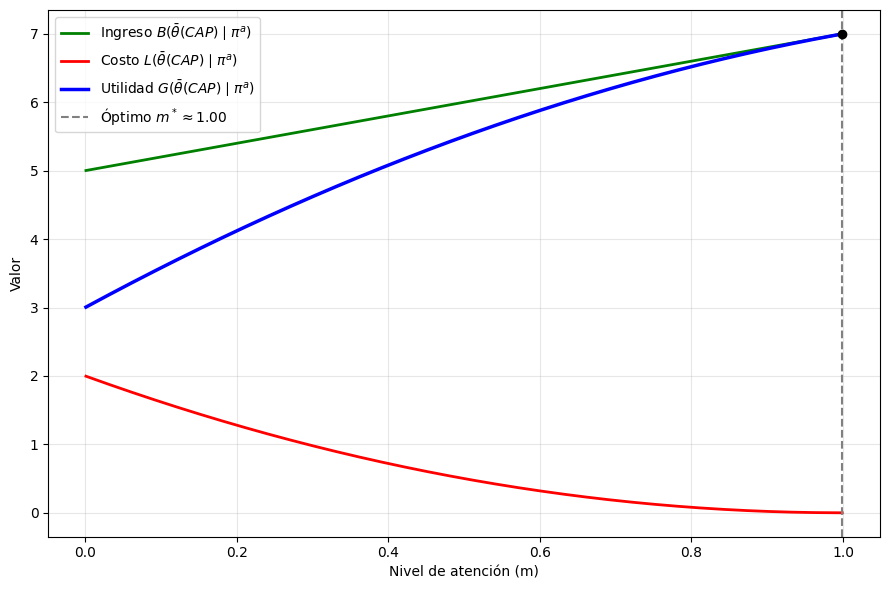
\includegraphics[width=0.75\linewidth]{figures/costo precisión gabaix.png}
%     \caption{Utilidad del planificador social con costo de precisión. (Fuente: elaboración propia)}
%     \label{fig:GX1}
% \end{figure}

% Al analizar la figura \ref{fig:GX1} se puede notar que la función de costos penaliza por la imprecisión, es decir al comenzar en $m=0$ y $\theta=5$ era alto el costo, luego al mejorar su nivel de atención el costo es cada vez menor hasta llegar a atención perfecta $m=1$ donde $\theta = CAP$. Tener atención perfecta no es viable en el mundo real y el modelo falla al no castigar por esto. 

% Se describe entonces una forma de incorporar un castigo por obtener atención perfecta ($m=1$) que es precisamente el costo que presenta \citeA{gabaix_behavioral_2019} en el ejercicio de la sección 6.2.2 formulado en la ecuación \ref{eq:costosims}, un costo por procesar información.

% Primero analizaremos como se comporta este costo en la función objetivo sin incorporar todavía al costo $L(\bar{\theta}(CAP) \mid \pi^a)$.


% Puede verse que el planificador social puede tener información perfecta, lo que quiere decir que el sujeto tiene una CAPacidad grande para procesar a información. esto puede limitarse agregando la restricón de CAPacidad presente en la sección 6.2 del CAPitulo 4 de \citeA{gabaix_behavioral_2019}:
% \begin{equation}
%     \frac{1}{2} \log\left( \frac{1}{1 - m} \right) \leq K
%     \label{eq:restCAPacidad}
% \end{equation}

% Con la restricción \ref{eq:restCAPacidad} podemos graficar nuevamente el problema asumiendo una CAPacidad $K=0,9$. Véase la figura \ref{fig:kapparest}.


% \begin{figure}[H]
%     \centering
%     \includegraphics[width=0.75\linewidth]{restkappa.png}
%     \caption{Utilidad del planificador social con restricción de CAPacidad (Fuente: elaboración propia)}
%     \label{fig:kapparest}
% \end{figure}

% Se puede ver en la figura \ref{fig:kapparest} el planificador social no puede seguir adquiriendo información debido a su limitada CAPacidad. Por lo que intentara mejorar su precisión acercándose al CAP hasta el punto de que sus habilidades, herramientas, dinero u otro le permitan. 

% %Esto es más realista ya que es cada vez más costoso adquirir información e imposible tener la totalidad de esta. Las variables para estimar correctamente un CAP son muchas, la CAPacidad de las maquinas de medición, las áreas donde se mide, la necesidad eléctrica futura, entre muchas más, y esta es una manera de representar esos limites.




\section{Metodología para el establecimiento del presupuesto nacional}
\label{metodologiaAG}
La metodología utilizada para el sector energético en \citeA{gobierno_de_chile_estrategia_2021} se divide en 7 etapas de la letra A a la G mostradas a continuación:

\begin{itemize}
    \item \textbf{Etapa A: Escenario Base} \\
    Se proyectan variables macro y microeconómicas (PIB, población, costos tecnológicos y demanda de servicios energéticos). A partir de ello se estima la demanda energética y las emisiones bajo el escenario con políticas actuales.

    \item \textbf{Etapa B: Propuesta de Mitigación} \\
    Se definen y combinan distintas opciones de mitigación (cambios tecnológicos, eficiencia energética, gestión de demanda y sustitución de energías) para generar escenarios alternativos.

    \item \textbf{Etapa C: Modelos Sectoriales} \\
    El sector eléctrico se modela mediante optimización de menor costo. Los sectores no eléctricos se simulan asignando tecnologías y estimando sus costos como costo por tecnología multiplicado por la demanda.

    \item \textbf{Etapa D: Curvas MAC} \\
    Se construyen curvas de costo marginal de abatimiento (MAC) a partir de los costos y emisiones del escenario base, para ordenar y priorizar las medidas de mitigación según su costo/efectividad.

    \item \textbf{Etapa E: Emisiones Nacionales} \\
    Se integran las emisiones del sector energía con las de los sectores no energéticos, obteniéndose la proyección total de emisiones nacionales de GEI.

    \item \textbf{Etapa F: Confrontación con la Meta} \\
    Las emisiones proyectadas se comparan con la meta de neutralidad al 2050, considerando una captura del sector UTCUTS de 65 MtCO$_2$eq. Si no se cumple la meta se repite el proceso aumentando la ambición; si se cumple, se optimizan los costos.

    \item \textbf{Etapa G: Propuesta Final de la NDC} \\
    El proceso finaliza cuando se logra la neutralidad al menor costo posible. Las medidas resultantes constituyen la base de la propuesta de mitigación de la NDC.
     
\end{itemize}

% \section{Presupuestos de emisión históricos}
% \begin{flushleft}
% \footnotesize
% \textbf{Fuentes:}
% \begin{itemize}
%     \item Climate Action Tracker: \url{https://climateactiontracker.org/}
%     \item Climate Action Tracker (CFI): \url{https://climateactiontracker.org/}
%     \item White Paper NDC (2019): Mitigation\_NDC\_White\_Paper.pdf
%     \item Propuesta metodológica GEI (MMA, 2021): 
%     \url{https://cambioclimatico.mma.gob.cl/wp-content/uploads/2020/07/Minuta-Metodologia-Presupuestos-carbono-sectoriales.pdf}
%     \item PAMCC (2024): \url{https://cambioclimatico.mma.gob.cl/}
%     \item MMA (2024): \url{https://cambioclimatico.mma.gob.cl/}
%     \item Anteproyecto actualización NDC (2025)
% \end{itemize}
% \end{flushleft}




















% \begin{table}[H]
% \centering
% \caption{Distancia absoluta entre la participación solar simulada y la observada (2023) bajo distintos niveles de atención y escenarios}
% \label{tab:solar_distancia_completa}
% \renewcommand{\arraystretch}{1,1}
% \setlength{\tabcolsep}{6pt}
% \small
% \begin{tabular}{c c c c c}
% \toprule
% \textbf{$m$} &
% \textbf{Escenario} &
% \textbf{Solar modelo (\%)} &
% \textbf{Solar real (\%)} &
% \textbf{Distancia absoluta (\%)} \\
% \midrule
% 0,0 & 5 & 19,81 & 19,70 & 0,11 \\
% 0,1 & 5 & 20,09 & 19,70 & 0,39 \\
% 0,2 & 5 & 20,38 & 19,70 & 0,68 \\
% 0,3 & 5 & 20,66 & 19,70 & 0,96 \\
% 0,4 & 5 & 20,95 & 19,70 & 1,25 \\
% 0,5 & 5 & 21,23 & 19,70 & 1,53 \\
% 0,6 & 5 & 21,51 & 19,70 & 1,81 \\
% 0,0 & 1 & 21,58 & 19,70 & 1,88 \\
% 0,1 & 1 & 21,78 & 19,70 & 2,08 \\
% 0,0 & 3 & 21,78 & 19,70 & 2,08 \\
% 0,7 & 5 & 21,80 & 19,70 & 2,10 \\
% 0,2 & 1 & 21,98 & 19,70 & 2,28 \\
% 0,1 & 3 & 21,98 & 19,70 & 2,28 \\
% 0,8 & 5 & 22,08 & 19,70 & 2,38 \\
% 0,3 & 1 & 22,17 & 19,70 & 2,47 \\
% 0,2 & 3 & 22,17 & 19,70 & 2,47 \\
% 0,9 & 5 & 22,29 & 19,70 & 2,59 \\
% 0,4 & 1 & 22,37 & 19,70 & 2,67 \\
% 0,3 & 3 & 22,37 & 19,70 & 2,67 \\
% 0,0 & 2 & 22,49 & 19,70 & 2,79 \\
% 1,0 & 5 & 22,49 & 19,70 & 2,79 \\
% 0,5 & 1 & 22,57 & 19,70 & 2,87 \\
% 0,4 & 3 & 22,57 & 19,70 & 2,87 \\
% 0,1 & 2 & 22,64 & 19,70 & 2,94 \\
% 0,6 & 1 & 22,76 & 19,70 & 3,06 \\
% 0,5 & 3 & 22,77 & 19,70 & 3,07 \\
% 0,2 & 2 & 22,79 & 19,70 & 3,09 \\
% 0,3 & 2 & 22,94 & 19,70 & 3,24 \\
% 0,7 & 1 & 22,96 & 19,70 & 3,26 \\
% 0,6 & 3 & 22,96 & 19,70 & 3,26 \\
% 0,4 & 2 & 23,09 & 19,70 & 3,39 \\
% 0,8 & 1 & 23,16 & 19,70 & 3,46 \\
% 0,7 & 3 & 23,16 & 19,70 & 3,46 \\
% 0,5 & 2 & 23,24 & 19,70 & 3,54 \\
% 0,0 & 4 & 23,33 & 19,70 & 3,63 \\
% 0,9 & 1 & 23,35 & 19,70 & 3,65 \\
% 0,8 & 3 & 23,36 & 19,70 & 3,66 \\
% 0,6 & 2 & 23,39 & 19,70 & 3,69 \\
% 0,1 & 4 & 23,48 & 19,70 & 3,78 \\
% 0,9 & 3 & 23,52 & 19,70 & 3,82 \\
% 0,7 & 2 & 23,54 & 19,70 & 3,84 \\
% 1,0 & 1 & 23,55 & 19,70 & 3,85 \\
% 0,2 & 4 & 23,62 & 19,70 & 3,92 \\
% 1,0 & 3 & 23,68 & 19,70 & 3,98 \\
% 0,8 & 2 & 23,70 & 19,70 & 4,00 \\
% 0,3 & 4 & 23,76 & 19,70 & 4,06 \\
% 0,9 & 2 & 23,85 & 19,70 & 4,15 \\
% 0,4 & 4 & 23,90 & 19,70 & 4,20 \\
% 1,0 & 2 & 24,00 & 19,70 & 4,30 \\
% 0,5 & 4 & 24,04 & 19,70 & 4,34 \\
% 0,6 & 4 & 24,18 & 19,70 & 4,48 \\
% 0,7 & 4 & 24,32 & 19,70 & 4,62 \\
% 0,8 & 4 & 24,48 & 19,70 & 4,78 \\
% 0,9 & 4 & 24,65 & 19,70 & 4,95 \\
% 1,0 & 4 & 24,82 & 19,70 & 5,12 \\
% \bottomrule
% \end{tabular}




% \vspace{0,1cm}
% \footnotesize{\textit{Nota:} La distancia absoluta se calcula como 
% $\left| \text{Solar modelo} - \text{Solar real} \right|$.  
% Fuente: Elaboración propia.}
% \end{table}



% \begin{table}[H]
% \centering
% \small
% \caption{Distancia absoluta entre el mix tecnológico modelado y el observado (parte I)}
% \label{tab:distancia_mix_completa_1}
% \renewcommand{\arraystretch}{1.1}
% \setlength{\tabcolsep}{6pt}
% \begin{tabular}{c c c}
% \toprule
% \textbf{$m$} & \textbf{Escenario} & \textbf{Distancia absoluta} \\
% \midrule
% 0.0 & 5 & 0.2727 \\
% 0.1 & 5 & 0.2758 \\
% 0.2 & 5 & 0.2788 \\
% 0.3 & 5 & 0.2818 \\
% 0.4 & 5 & 0.2849 \\
% 0.0 & 1 & 0.2875 \\
% 0.5 & 5 & 0.2879 \\
% 0.1 & 1 & 0.2903 \\
% 0.6 & 5 & 0.2909 \\
% 0.2 & 1 & 0.2937 \\
% 0.7 & 5 & 0.2940 \\
% 0.0 & 3 & 0.2945 \\
% 0.8 & 5 & 0.2970 \\
% 0.3 & 1 & 0.2994 \\
% 0.9 & 5 & 0.2998 \\
% 0.1 & 3 & 0.3015 \\
% 1.0 & 5 & 0.3026 \\
% 0.0 & 2 & 0.3072 \\
% 0.4 & 1 & 0.3087 \\
% 0.2 & 3 & 0.3109 \\
% 0.1 & 2 & 0.3134 \\
% 0.5 & 1 & 0.3181 \\
% 0.2 & 2 & 0.3195 \\
% 0.3 & 3 & 0.3202 \\
% 0.3 & 2 & 0.3257 \\
% 0.6 & 1 & 0.3274 \\
% 0.4 & 3 & 0.3295 \\
% 0.4 & 2 & 0.3318 \\
% \bottomrule
% \end{tabular}

% \vspace{0.15cm}
% \footnotesize{Fuente: Elaboración propia.}
% \end{table}




% \begin{table}[H]
% \centering
% \small
% \caption{Distancia absoluta entre el mix tecnológico modelado y el observado (parte II)}
% \label{tab:distancia_mix_completa_2}
% \renewcommand{\arraystretch}{1.1}
% \setlength{\tabcolsep}{6pt}
% \begin{tabular}{c c c}
% \toprule
% \textbf{$m$} & \textbf{Escenario} & \textbf{Distancia absoluta} \\
% \midrule
% 0.7 & 1 & 0.3368 \\
% 0.5 & 2 & 0.3379 \\
% 0.5 & 3 & 0.3389 \\
% 0.0 & 4 & 0.3428 \\
% 0.6 & 2 & 0.3441 \\
% 0.8 & 1 & 0.3461 \\
% 0.6 & 3 & 0.3482 \\
% 0.1 & 4 & 0.3487 \\
% 0.7 & 2 & 0.3502 \\
% 0.2 & 4 & 0.3545 \\
% 0.9 & 1 & 0.3554 \\
% 0.8 & 2 & 0.3564 \\
% 0.7 & 3 & 0.3576 \\
% 0.3 & 4 & 0.3600 \\
% 0.9 & 2 & 0.3625 \\
% 1.0 & 1 & 0.3648 \\
% 0.4 & 4 & 0.3654 \\
% 0.8 & 3 & 0.3669 \\
% 1.0 & 2 & 0.3687 \\
% 0.5 & 4 & 0.3707 \\
% 0.9 & 3 & 0.3734 \\
% 0.6 & 4 & 0.3760 \\
% 1.0 & 3 & 0.3800 \\
% 0.7 & 4 & 0.3813 \\
% 0.8 & 4 & 0.3882 \\
% 0.9 & 4 & 0.3958 \\
% 1.0 & 4 & 0.4034 \\
% \bottomrule
% \end{tabular}

% \vspace{0.15cm}
% \footnotesize{Fuente: Elaboración propia.}
% \end{table}


\section{Parámetros originales de \protect\citeA{amigo_two_2021}}
\begin{table}[H]
\centering
\caption{Factores de planta por tecnología}
\label{tab:factor_planta}
\renewcommand{\arraystretch}{1.2}
\setlength{\tabcolsep}{14pt}
\begin{tabular}{l c}
\toprule
\textbf{Tecnología} & \textbf{Factor de planta (CF)} \\
\midrule
Biomasa           & 0.55 \\
Carbón            & 0.99 \\
Eólica            & 0.23 \\
Gas               & 0.60 \\
Geotérmica        & 0.65 \\
Hidro Embalse     & 0.39 \\
Hidro Pasada      & 0.43 \\
Hidro Mini Pasada & 0.39 \\
Petróleo Diésel   & 0.90 \\
Solar             & 0.24 \\
\bottomrule
\end{tabular}

\vspace{0.1cm}
\footnotesize{Fuente: elaboración propia en base a el trabajo de \citeA{amigo_two_2021}.}
\end{table}
\begin{table}[H]
\centering
\caption{Costos de inversión por tecnología}
\label{tab:inv_cost}
\renewcommand{\arraystretch}{1.2}
\setlength{\tabcolsep}{14pt}
\begin{tabular}{l c}
\toprule
\textbf{Tecnología} & \textbf{Costo de inversión (USD/kW)} \\
\midrule
Biomasa            & 3\,253 \\
Carbón             & 3\,000 \\
Eólica             & 1\,361 \\
Gas                & 800 \\
Geotérmica         & 5\,870 \\
Hidro Embalse      & 2\,180 \\
Hidro Pasada       & 4\,050 \\
Hidro Mini Pasada  & 3\,565 \\
Petróleo Diésel    & 687 \\
Solar              & 2\,000 \\
\bottomrule
\end{tabular}

\vspace{0.1cm}
\footnotesize{Fuente: elaboración propia en base a el trabajo de \citeA{amigo_two_2021}.}
\end{table}

\begin{table}[H]
\centering
\caption{Factores de emisión por tecnología}
\label{tab:epsilon}
\renewcommand{\arraystretch}{1.2}
\setlength{\tabcolsep}{14pt}
\begin{tabular}{l c}
\toprule
\textbf{Tecnología} & \textbf{Factor de emisión $\epsilon_i$ (tCO$_2$e/MWh)} \\
\midrule
Biomasa            & 0.00 \\
Carbón             & 0.91 \\
Eólica             & 0.00 \\
Gas                & 0.65 \\
Geotérmica         & 0.00 \\
Hidro Embalse      & 0.00 \\
Hidro Pasada       & 0.00 \\
Hidro Mini Pasada  & 0.00 \\
Petróleo Diésel    & 0.91 \\
Solar              & 0.00 \\
\bottomrule
\end{tabular}

\vspace{0.1cm}
\footnotesize{Fuente: elaboración propia en base a el trabajo de \citeA{amigo_two_2021}.}
\end{table}













































